\documentclass[12pt,conference]{IEEEtran}
\usepackage[utf8]{inputenc}
\usepackage{cite}
\usepackage{amsfonts}
\usepackage[pdftex]{graphicx}
\usepackage{array}
\usepackage{caption}
\usepackage{listings}
\usepackage{color}
\usepackage{float}
\hyphenation{op-tical net-works semi-conduc-tor}

\definecolor{codegreen}{rgb}{0,0.6,0}
\definecolor{codegray}{rgb}{0.5,0.5,0.5}
\definecolor{codepurple}{rgb}{0.58,0,0.82}
\definecolor{backcolour}{rgb}{0.98,0.98,0.97}
\lstdefinestyle{mystyle}{
	backgroundcolor=\color{backcolour},   
	commentstyle=\color{codegreen},
	keywordstyle=\color{magenta},
	numberstyle=\tiny\color{codegray},
	stringstyle=\color{codepurple},
	basicstyle=\footnotesize\ttfamily,
	breakatwhitespace=false,         
	breaklines=true,                 
	captionpos=b,                    
	keepspaces=true,                 
	numbers=left,                    
	numbersep=7pt,                  
	showspaces=false,                
	showstringspaces=false,
	showtabs=false,                  
	tabsize=2,
	frame=single,
	framerule=0pt,
	framesep=5pt,
	xleftmargin=.015\textwidth, xrightmargin=.015\textwidth
}
\lstset{language=C, style=mystyle}

\begin{document}

\title{Vulkan based volume rendering\\using ray tracing}

\author{\IEEEauthorblockN{Yanick Lukic}
\IEEEauthorblockA{Zurich University of Applied Sciences, Winterthur, Switzerland\\
Email: yanick.lukic@gmail.com}}
\maketitle
\thispagestyle{plain}
\pagestyle{plain} 

\begin{abstract}
The visualization of volumetric data becomes more and more a crucial part in different scientific domains.
To date it is not possible to visualize large data sets (multiple giga to tera bytes) at a real-time rate (e.g. 60 frames per seconds).
This work focuses on the rendering part and the data structure needed in a rendering system by introducing a basic list-based representation for an octree, that is directly compatible with the SPIR-V shader environment. For further investigations a ray tracer is implemented using the Vulkan API.
Building on a compute shader approach we are able to render small volumetric data sets in real time, although without a fully optimized ray tracer. Problems arise when data sets exceed the on-board memory of the GPU.
The presented data structure can not be used as is for a dynamic memory model between the CPU and the GPU, and needs further modifications to deal with the issue of large data sets.
\end{abstract}

\section{Introduction and related work}
Visualizing volumetric data is an elementary part in many scientific domains, such as biology, medicine and physics. The hardware improvements of the last two decades enable massive parallel computing on GPUs and make it possible to visualize complex volume data using the ray tracing algorithm\cite{purcell2002ray}. Even though this approach can be highly parallelized, current work is not able to render the pure data of big data sets in real-time (e.g. more than 60 frames per second). However, this algorithm is heavily dependent on the on-board memory size of the GPU. Systems like the Tuvok architecture make use of sophisticated methods to generate a compressed multiresolution hierarchy of the data set. Well reasoned paging heuristics and the use of data bricking enable them to quickly load the needed data for the next frame\cite{fogal2010tuvok}. Although, the Tuvok architecture is able to process big volumetric data sets, it is built to deliver a high quality final frame and does not achieve smooth transitions between different levels of detail while the user interacts with the data set. This makes the Tuvok architecture as it stands not usable for applications where throughout a high number of frames per second is needed to ensure a good interactivity for a user, e.g. when used with virtual reality.
\par
Other approaches rely on advanced compression algorithms. The compressed data is then decompressed at rendering time. Thereby the renderer can often be used as a single-pass volume renderer\cite{guthe2002interactive}. On the downside this approach does not scale up to very large data sets, since even the compressed data exceeds the available on-board memory of the GPU at a certain point.
\par
Additionally, recent work studied different tensor approximation models to compress the data used for volume rendering\cite{ballester2015analysis}. Even though these approaches are loss-bearing, they seem promising as a supplementary tool for handling large data sets. 
\par
Very good results are achieved by using big GPU clusters to parallelize the large data and handle the calculation effort needed, as in \cite{nvidia2014index}. In contrast, our research focuses on single GPU systems, to ensure a compatibility with consumer level hardware.
\par
The best results on a single GPU to our knowledge are achieved by the GigaVoxels rendering pipeline\cite{crassin2009gigavoxels}. It is based on sparse octree ray-casting and is able to render data sets that exceed the GPUs on-board memory at interactive or even real-time performance.
\par
For a more detailed overview of the current state of the art in the area of GPU techniques for visualizing large data sets we refer to \cite{beyer2014survey}.
\par
The remainder of this paper is organized as follows. In section \ref{approach} we describe our setup of the Vulkan Pipeline and our newly designed data structure. To demonstrate the possibilities of our prototype we show some rendering results of different test data sets in section \ref{results}. The paper concludes with a summary and future research directions in section \ref{conclusion}.

\section{Approach}
\label{approach}
We separate the described problem into two major sub-issues, the rendering and the data-management. In this work we focus on the rendering part of volumetric data using an improved ray tracing algorithm. For this we develop an octree based data structure which can be easily processed by the GPU.  

\subsection{Vulkan implementation}
We use the new Vulkan API as a basis for our prototype. With this we prepare for the massive data handling in later work. The main reason for using Vulkan is its ability to avoid CPU overhead\cite{vulkan1.0.38spec}, which can be the case when working with large data sets that do not fit into the GPUs on-board memory.
\par
Vulkan is extremely initialization heavy. Therefore the whole graphics pipeline has to be explicitly defined. 

First, the basic components needed by the graphics pipeline are created. Starting with the command buffers. Command buffer objects are recorded operations that have to be performed. They allow for parallel preparation of commands which then can be executed in the main loop. To setup the command buffers, a command pool is initialized which manages the memory from which the command buffers are then allocated..

The second component is the swap chain. It refers to a set of images to render to which can then be presented to the windowing system. For each swap chain image a command buffer is created, that can be reused for rendering commands.

Further, the render pass created. That is an object which holds the framebuffers attachments needed by the different pipeline stages.

The graphics pipeline needs memory to execute commands, for that a pipeline cache is created.

To draw the images from the swap chain on the screen they have to be referenced as attachments by a framebuffer. Therefore we create a framebuffer for each swap chain image.

Next, the uniform buffer objects (UBOs) and the shader storage buffer objects (SSBOs) are initialized. They hold the entire data of the scene, e.g. the voxel data set and the viewers position. As a next step, the texture target of the renderer is defined, this serves as the actual rendering target of the ray tracer.
\par
Subsequently, the actual graphics pipeline is defined. This includes the specification of all pipeline-stages. Shader stages are modules that define the programmable stages of the graphics pipeline, like the vertex and the fragment shader. The fixed function stages can not be programmed but their behavior needs to be explicitly defined (e.g. input assembly, rasterizer, viewport and color blending). Additionally the pipeline layout needs to be defined, which are the resource descriptors of the shaders. These descriptor sets enable the shaders to access resources like buffers and images. Further the render pass is added to the pipeline. 
Even though the graphics pipeline is necessary, it is not as important for our system. The reason for this is that the rendering process takes place in a compute shader, the generated texture is then projected on a fixed plane, that is statically positioned in front of the viewer. The computational part is separated from the graphics pipeline and has therefore its own pipeline, which is defined later.
\par
The initialization process continues by declaring a descriptor pool. Descriptor sets can not be created directly, they need to be allocated from a descriptor pool. The descriptor sets defined in the pipeline can now be allocated.
\par
After this, the compute pipeline is set up. Overall a very similar process to the graphics pipeline except there are no stages beside one compute shader. To keep the two pipelines separated, we use an additional command pool for the compute pipeline. The actual rendering performed in the compute shader is explained in detail in section \ref{sec:renderer}. 
\par
Now we are able to use command buffers of the graphics pipeline to execute render passes. These are synchronized with the commands of the compute pipeline which create the actual rendered image, that is then delivered to the screen.
\par
For further reading about the Vulkan API we refer to the official specification\cite{vulkan1.0.38spec} and an excellent tutorial from Alexander Overvoorde\cite{overvoorde2016vulkan}.
\par
To handle the windowing and input system of the operation system we use the \texttt{GLFW} library\cite{loewy2016glfw}. Additionally, we use the \texttt{GLM} library\cite{creation2016glm} to ensure our datatypes in the C++ code are shader compatible.

\subsection{Datastructure}
To enable efficient raytracing, binary partitioning methods, such as binary space partinioning trees (BSP-trees), are needed. We use an octree introduced in \cite{meagher1982geometric} as data structure. Even though, KD-trees are better suited for fast raytracing\cite{havran2000heuristic}, we have to keep the limited on-board memory of the GPU in mind. Octrees are highly structured and predictable which allows for optimization in the data structure\cite{crassin2009gigavoxels}.
Hence, the octree serves as a basis for our data structure. To calculate the number of nodes in the octree, equation \ref{octree_size} can be used. Thereby $N$ terms the number of voxel points in the volume, aligned in a cubic grid.
\begin{equation} 
O = \sum\limits_{p=0}^{n} 8^{p} \quad \textrm{with} \quad n = \frac{\log(N)}{\log(8)}
\label{octree_size} 
\end{equation}

We use a list of voxels as the raw input data for our data structure. The list needs to be of length $2^p$ with $p \in \mathbb{N}$. To build the octree from this list we have to extract all the siblings blockwise. To achieve this we use a static algorithm which is described in listing \ref{lst:siblings}.

\begin{lstlisting}[label=lst:siblings, caption={To find the siblings of a given voxel inside the input list we use this static algorithm. Aside from the index of the first voxel we also need the side length of the cubic volume, labeled as $N$ in the above listing.}]
voxelIndices[0] = startIdx;
voxelIndices[1] = startIdx + 1;
voxelIndices[2] = startIdx + N;
voxelIndices[3] = startIdx + N + 1;
voxelIndices[4] = startIdx + N^2;
voxelIndices[5] = startIdx + N^2 + 1;
voxelIndices[6] = startIdx + N^2 + N;
voxelIndices[7] = startIdx + N^2 + N + 1;
\end{lstlisting}

Furthermore it is necessary to determine which is the start index of the next block of siblings. This is particularly more complex than determining which the siblings are. Because there are three different cases: First, the next block can be reached by increasing the $x$-axis. Second, adjusting the $x$- and $y$-axis is necessary, in this case the next block is a row further up. And lastly, the next block can only be reached by adjusting all axis, this is the case when all rows of one layer are processed. The used code is visualized in listing \ref{lst:nextblock}.
\begin{lstlisting}[label=lst:nextblock, caption={Finding the next block start index needs to cover three cases.}]
int nextIdx = currentIdx + 2;
// + 2 because zero based index
if ((currentIdx+2) mod N == 0) {
	nextIdx += N;
	if (((currentIdx+2)/N+1) mod N==0) {
		nextIdx += N*N;
	}
}
return nextIdx
\end{lstlisting}

Combining the algorithms from listings \ref{lst:siblings} and \ref{lst:nextblock} allows extracting all sibling blocks for the octree from bottom up.

\par

Standard octree implementations use references such as pointers to reference the children of a node. Because we want to use the data structure on the GPU we have two options. Hand the data over as textures (1D, 2D or 3D) or hand over an array containing all the nodes. Even though, using textures would benefit from texture interpolation implemented in hardware, we chose the latter approach. The reason was mainly the simplicity of the prototype. To work with a single list we need to determine how the nodes are arranged inside that list and which information each node needs that traversing the octree becomes possible. One node in our prototype uses $4$ bytes for color encoding and $4$ bytes for storing an index to the first child. This basic node structure needs all children of a node to be placed together in one block. As shown in fig. \ref{fig:datastructure} the octree is built from left to right, means the first node in the list corresponds to the root node of the octree. 
\begin{figure*}[htp]
	\centering
	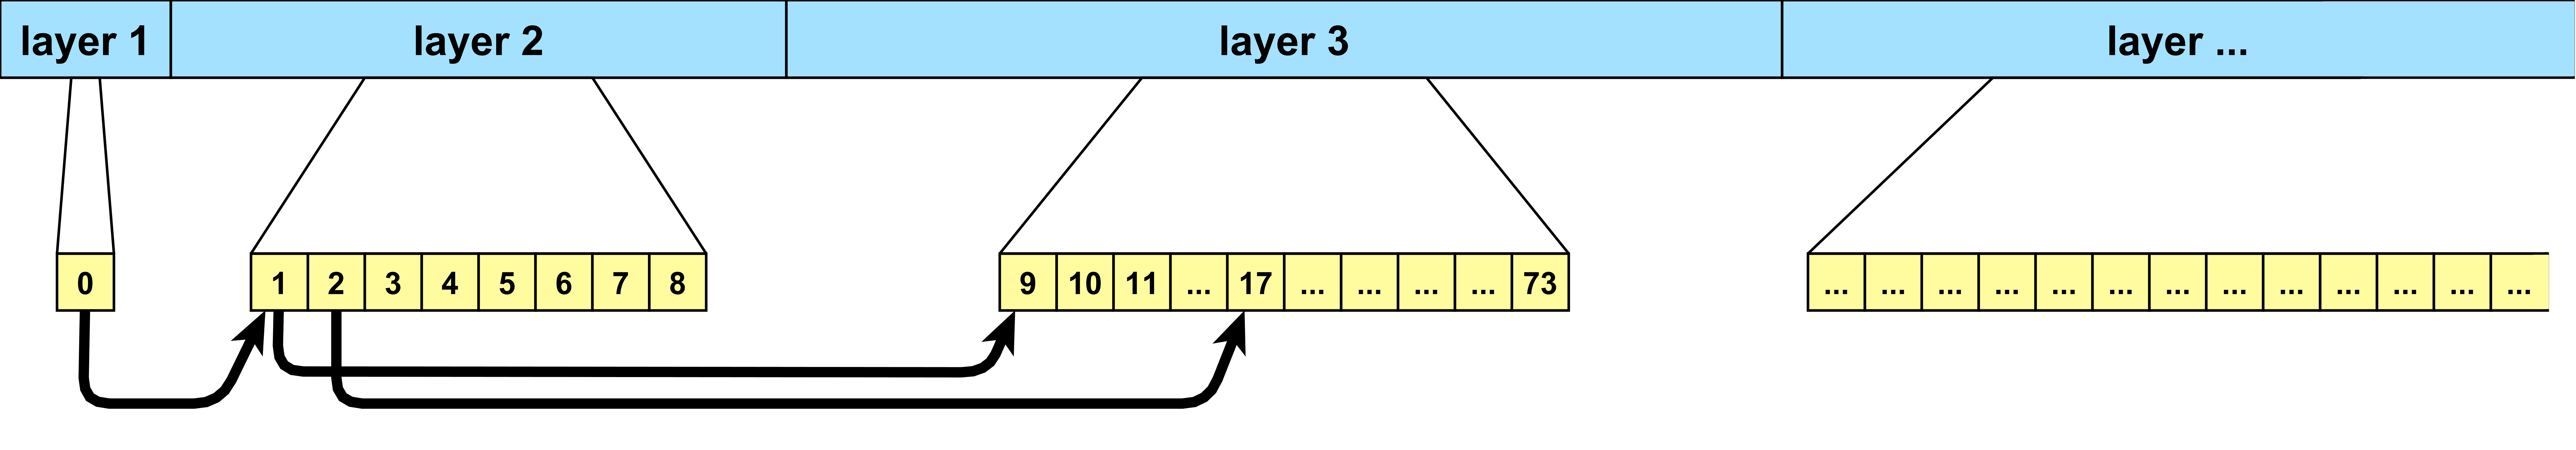
\includegraphics[width=0.8\textwidth]{images/datastructure.png}
	\caption{The structure of the octree represented by a single list.}
	\label{fig:datastructure}
\end{figure*}
The data structure is created \textit{a priori} and then handed over to the GPU. After that the whole rendering process takes place on the GPU.

\subsection{Renderer}
\label{sec:renderer}
The renderer is implemented as a compute shader. We used the GLSL interface for SPIR-V for coding. As shown in fig. \ref{fig:renderingprocess} the shader uses the octree data and additional attributes as input. To hand over data to the GPU there are two possibilities: uniform buffer objects (UBOs) and shader storage buffer objects (SSBOs)\cite{vulkan1.0.38spec}. Dependent on the hardware for UBOs only a maximum size of $16$KB is guaranteed. For SSBOs the guaranteed maximum size is $16$MB, but on most modern GPUs it is roughly $2$GB\cite{willems2016vulkan}. For this reason we share the octree as an SSBO and the further meta information (e.g. octree position) as an UBO.
\par
Once the data is fed to the shader it produces an output image using a modified ray tracing algorithm. The image is then used as a texture and painted on the plane setup in front of the screen by the fragment shader. While rendering, the compute shader contains logic to evaluate the needed data resolution for a certain pixel and interrupts the ray tracing algorithm accordingly to lower the computational complexity effort. This process is executed highly parallel by calculating the pixel colors independently and therefore concurrently.

\begin{figure*}[htp]
	\centering
	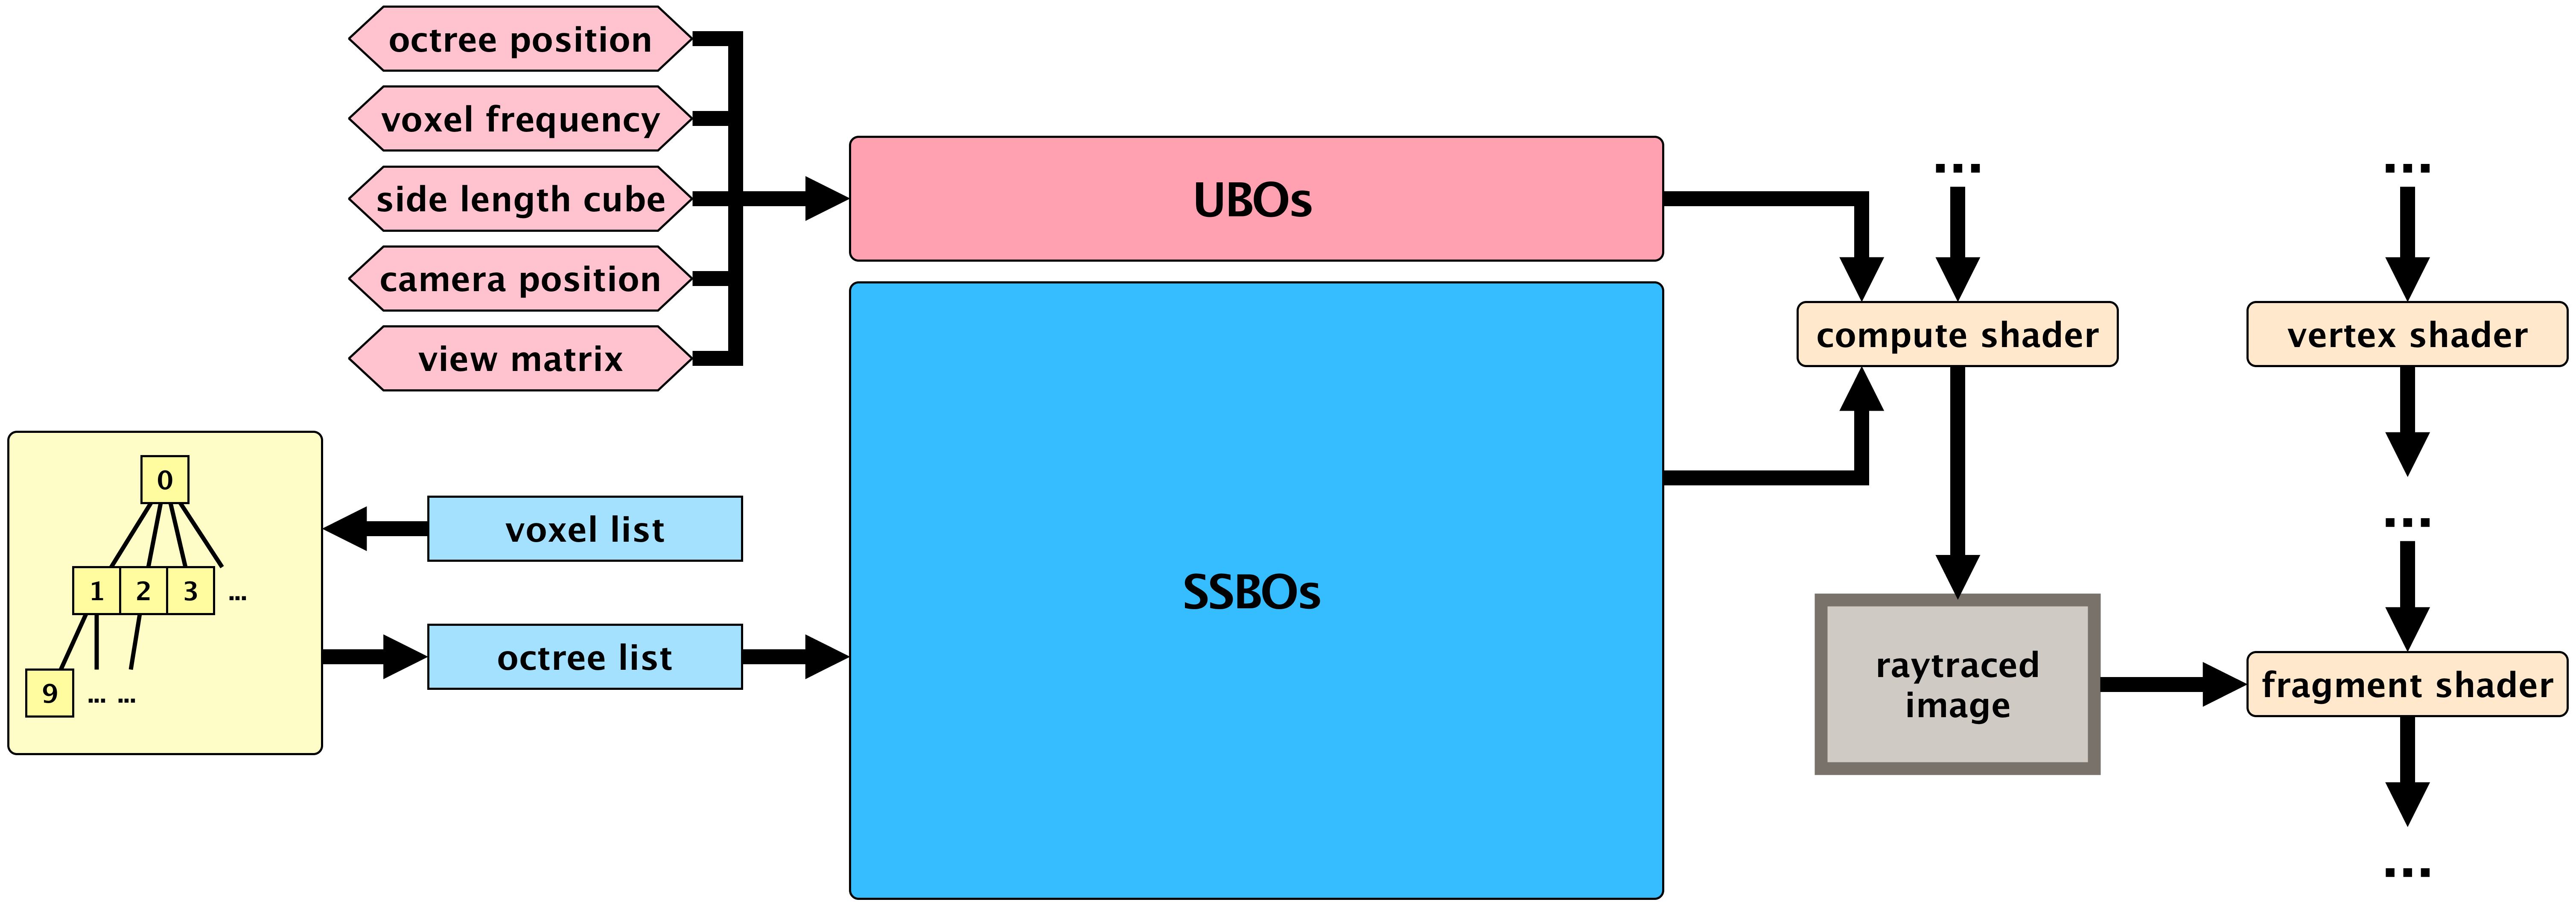
\includegraphics[width=0.8\textwidth]{images/rendering_process.png}
	\caption{The shown pipeline visualizes the core steps which are performed to render a single image and hand it to the fragment shader, which then paints it on the polygons in front of the camera.}
	\label{fig:renderingprocess}
\end{figure*}

As soon as a non-cubic volume is rendered, the octree contains transparent nodes. To handle this, not only the first node hit by the ray is needed, rather all nodes hit behind that node as long as the alpha value of the pixel color has not reached $1.0$ or the volume is passed. In the latter case the color is mixed with the background color, which is $rgb(0, 0, 0)$ (black).


\section{Results}
\label{results}
The octree enables the possibility of a dynamic level of detail. By that it is simple to adjust the current level of detail to the position of the viewer. Fig. \ref{fig:hierarchiesCube} shows the four hierarchical stages of a $32^3$ cube volume. 
\begin{figure}[htp]
	\centering
	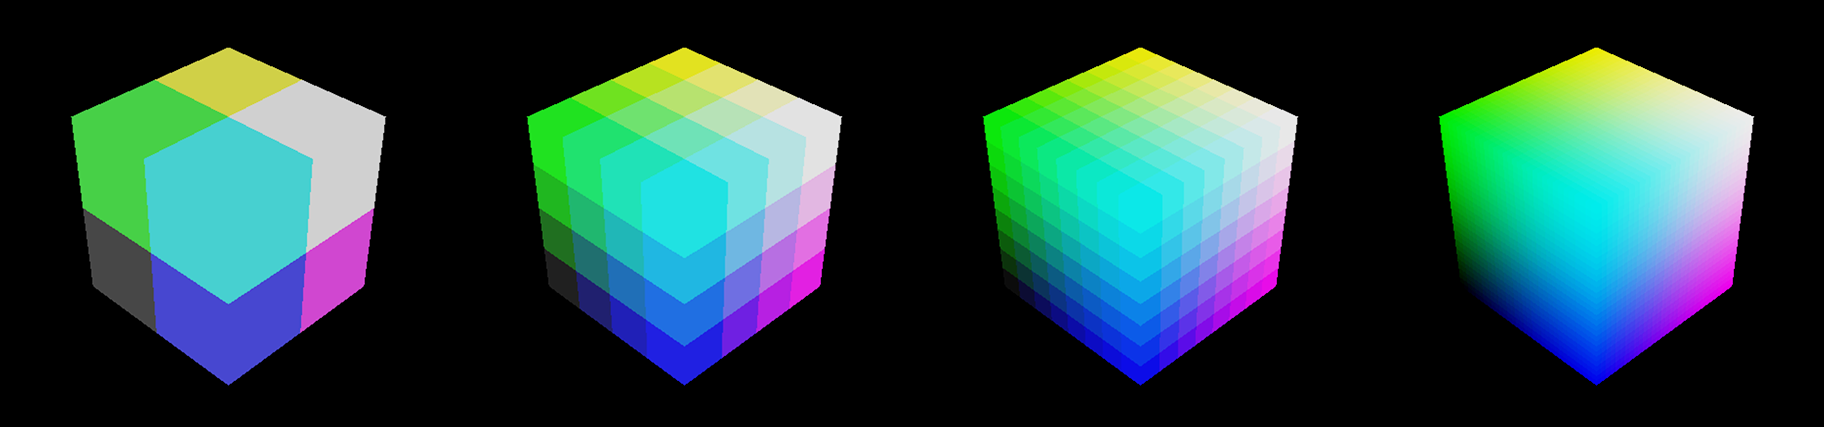
\includegraphics[width=0.4\textwidth]{images/cube_hierarchy.png}
	\caption{The different hierarchical stages of a $32^3$ cube volume.}
	\label{fig:hierarchiesCube}
\end{figure}

Switching between hierarchies has a significant impact on the achieved frames per second. This effect is dependent on the initial size of the data set (the bigger the data set the higher the impact on the frames per second). But even without suspending the traversal at a given stage and always stepping to the voxel data on the lowest layer, the performance benefit of the octree is significant. The reason for this is, that the traversal algorithm only needs to visit a fraction of the nodes.
\par
Our system is able to render complex data sets, as shown in fig. \ref{fig:kidneyRendering} where a data set of a mouse kidney with a $256^3$ resolution is rendered. The performance is dependent on the number of semi-transparent nodes in the octree as well as the position of the viewer, whereas the latter is the most important. For the above mentioned data set we achieve highly interactive frame rates when positioned at a medium distance (30-60 fps). The frame rate ranges heavily dependent how much of the view is filled with the volume, e.g. 15 (near) to 150 (far) fps. When rendered with only fully transparent and fully visible nodes the achieved rendering rates are always approx. 10\% higher than when rendered with nodes where the alpha value equals the gray scale value.
This results are achieved when using a NVIDIA GeForce GT 650M with 1024 MB of on-board memory. The resolution of the rendered image is set to $1024\times 768$.

\begin{figure}[htp]
	\centering
	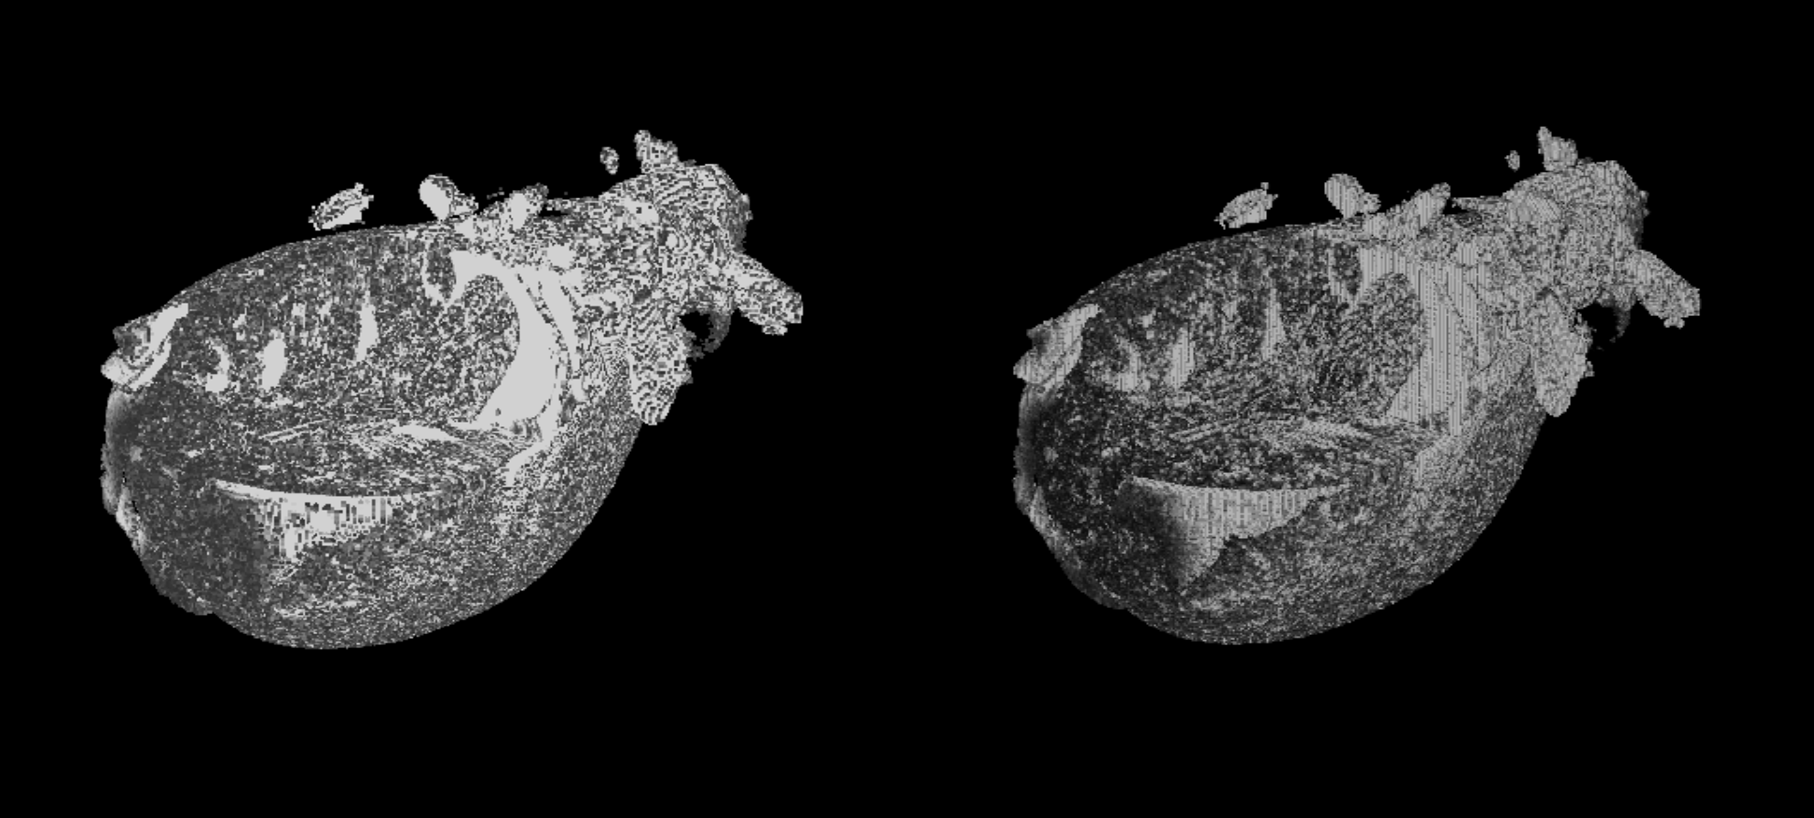
\includegraphics[width=0.45\textwidth]{images/kidney_256x256x256.PNG}
	\caption{Rendering of a mouse kidney at a resolution of $256^3$. Left with fully transparent or fully visible nodes. Right with nodes whose alpha value equals the gray scale value.}
	\label{fig:kidneyRendering}
\end{figure}

\section{Conclusion and future work}
\label{conclusion}
In this work we have implemented a prototype system investigating the volume rendering process using the ray tracing algorithm. The prototype is implemented using the Vulkan API with a compute shader as the actual renderer. We showed that it is crucial to use binary space partitioning methods. Without them it is not even possible to render small data sets (e.g. $8^3$) at an acceptable frame rate (over 20 fps). The octree is a powerful tool to achieve this, but with the weakness when rendering semi-transparent objects. But still, the ray tracing algorithm is pretty un-tuned and could be improved by adapting the fast voxel traversal algorithm described by Amanatides and Woo in \cite{amanatides1987fast} to our task. Furthermore, there are several possibilities to decrease the number of floating point operations inside the compute shader, e.g. to not check for every node whether it is behind the viewer instead using the information given by the parent. With this approaches we could further increase the current rendering performance of our prototype.
\par
Future work should consist of further developing the data structure. So it can be dynamically enhanced throughout the rendering process. This would address the problem of data sets that are too big for the on-board memory of the GPU. It should also be considered switching to work with textures instead of an array as representation of the octree. Reasons for this are mainly hardware-sided texture interpolation and the lack of dynamic indexing on the GPU.
%\par
%The open source code of the prototype is available at \texttt{https://github.com/yaluki/...}

\section{Acknowledgments}
The mouse kidney model is a courtesy of The Interface Group of the University of Zürich.

\bibliographystyle{IEEEtran}
\bibliography{mybib}
\end{document}


